%====================================================================================
\section{Segundo Teorema del Bienestar}
%====================================================================================

\begin{frame}{Segundo Teorema del Bienestar}
	\begin{itemize}
		\item Si tomamos una asignación eficiente, ¿podemos garantizar que esta sea de equilibrio competitivo?
		\item ``Cuando las preferencias de ambos consumidores son convexas, contínuas y monótonas, cualquier asignación óptimo de Pareto puede ser de equilibrio walrasiano, si se permite las adecuadas transferencias entre los consumidores''.
	\end{itemize}
\end{frame}
%------------------------------------------------
\begin{frame}{Segundo Teorema del Bienestar}
$X$	es una asignación óptima obtenida por equilibrio competitivo desde la dotación $W$.
	\begin{center}
		\vspace{-0.5cm}
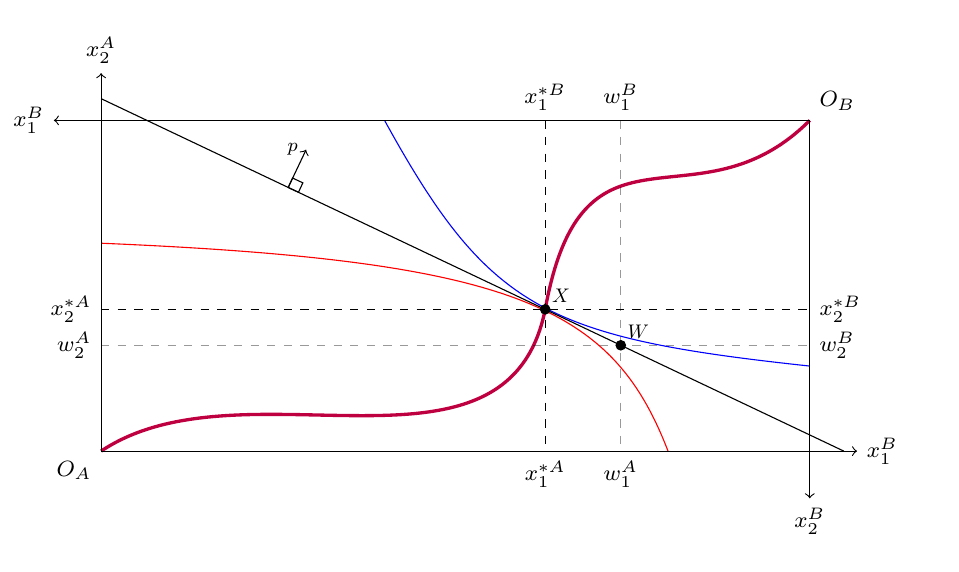
\begin{tikzpicture}[scale=1.2]
	\hspace{-0.3cm}
	% Curva de contrato 5.2,2
		\draw  [purple, very thick] (0.5,0.5) ..controls (2,1.5) and (4.8,0) .. (5.2,2) ..controls (5.6,4.2) and (6.8,2.8) .. (8,4);
	% Intersección de una dotación
		% Demanda: x
			\draw[dashed] (5.2,4) node[above] {\footnotesize $x_{1}^{*B}$} -- (5.2,0.5) node[below]{\footnotesize $x_{1}^{*A}$};
			\draw[dashed] (0.5,2) node[left] {\footnotesize $x_{2}^{*A}$} -- (8,2)node[right]{\footnotesize $x_{2}^{*B}$};
		
		% Oferta: w
			\draw[dashed, opacity=0.4] (6,4) -- (6,0.5);
			\draw[dashed, opacity=0.4] (0.5,1.62)  -- (8,1.62);
			
			\draw (8,1.62)  node [right] {\footnotesize $w_{2}^{B}$};
			\draw (6,4)  node [above] {\footnotesize $w_{1}^{B}$};
			
			\draw (0.5,1.62)  node [left] {\footnotesize $w_{2}^{A}$};
			\draw (6,0.5)  node [below] {\footnotesize $w_{1}^{A}$};
	
	% Curvas de indiferencia
		\draw [blue] (3.5,4) .. controls (4.6,2) and (5.2,1.7) .. (8,1.4);
		\draw [red] (0.5,2.7) .. controls (4.915,2.515) and (5.915,2.015) .. (6.5,0.5);
	
	% Recta presupuestaria
		\draw (0.5,4.23) -- (8.36,0.5);
	
	% Puntos
		\draw[black, fill=black] (5.2,2) circle[radius=0.05] node [above right, scale=0.25mm] {$X$};
		\draw[black, fill=black] (6,1.62) circle[radius=0.05] node [above right, scale=0.25mm] {$W$};
	
	% Flecha y rectángulo
		\draw [->] (2.48,3.29) -- (2.67,3.69) node [left, scale = 0.3mm] {\footnotesize $p$};
		\draw [rotate around={-25:(2.48,3.29)}] (2.48,3.29) rectangle (2.6, 3.4);
		
	% Formación de la caja
		% Consumidor A
			\draw[->] (0.5,0.5) node[align=center, below left] {\footnotesize $O_A$} -- (0.5,4.5) node[align=center, above] {\footnotesize $x_{2}^{A}$};
			\draw[->] (0.5,0.5) -- (8.5,0.5) node[align=center, right] {\footnotesize $x_{1}^{B}$};
		
		%Consumidor B
			\draw[->] (8,4) node[align=center, above right] {\footnotesize $O_B$} -- (0,4) node[align=center, left] {\footnotesize $x_{1}^{B}$};
			\draw[->] (8,4) -- (8,0) node[align=center, below] {\footnotesize $x_{2}^{B}$};
\end{tikzpicture}
	\end{center}
\end{frame}
%------------------------------------------------
\begin{frame}{Segundo Teorema del Bienestar}
¿Puede obtenerse esta asignación $N$ desde $W$? 
	\begin{center}
		\begin{tikzpicture}[scale=1]
	% Formación de la caja
	% Consumidor A
	\draw[->] (0.5,0.5) node[align=center, below left] {\footnotesize $O_A$} -- (0.5,4.5) node[align=center, above] {\footnotesize $x_{2}^{A}$};
	\draw[->] (0.5,0.5) -- (8.5,0.5) node[align=center, right] {\footnotesize $x_{1}^{A}$};
	
	\draw (6,0.5) node[below] {\footnotesize $x_{1}^{A}$};
	\draw (0.5,2) node[left] {\footnotesize $x_{2}^{A}$};
	
	% Llaves
	\draw [decorate,decoration={brace,amplitude=5pt},xshift=-4pt,yshift=0pt] (6.1,-0.05) -- (0.7,-0.05);
	\node [right] at (3,-0.4) {$w_{1}^{A}$};
	
	\draw [decorate,decoration={brace,amplitude=5pt},xshift=-4pt,yshift=0pt] (-0.05,0.5) --(-0.05,2);
	\node [left] at (-0.3,1.27) {$w_{2}^{A}$};
\end{tikzpicture}
	\end{center}
\end{frame}
%------------------------------------------------
\begin{frame}{Segundo Teorema del Bienestar}
¿Puede obtenerse esta asignación $N$ desde $W$? $\longrightarrow$ No, porque ya hay un sistema de precios y una dotación inicial
	\begin{center}
		\vspace{-0.5cm}
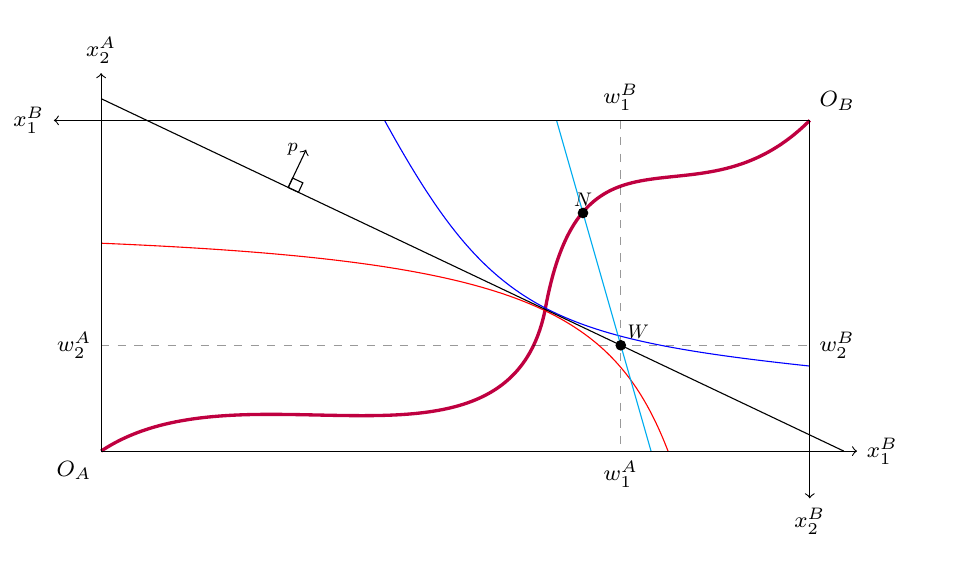
\begin{tikzpicture}[scale=1.2]
	\hspace{-0.3cm}
	% Curva de contrato 5.2,2
		\draw  [purple, very thick] (0.5,0.5) ..controls (2,1.5) and (4.8,0) .. (5.2,2) ..controls (5.6,4.2) and (6.8,2.8) .. (8,4);
	% Intersección de una dotación
		% Oferta: w
			\draw[dashed, opacity=0.4] (6,4) node [above, opacity=1] {\footnotesize $w_{1}^{B}$} -- (6,0.5) node [below, opacity=1] {\footnotesize $w_{1}^{A}$};
			\draw[dashed, opacity=0.4] (0.5,1.62)  node [left, opacity=1] {\footnotesize $w_{2}^{A}$} -- (8,1.62) node [right, opacity=1] {\footnotesize $w_{2}^{B}$};
	
	% Curvas de indiferencia
		\draw [blue] (3.5,4) .. controls (4.6,2) and (5.2,1.7) .. (8,1.4);
		\draw [red] (0.5,2.7) .. controls (4.915,2.515) and (5.915,2.015) .. (6.5,0.5);
	
	% Recta presupuestaria
		\draw (0.5,4.23) -- (8.36,0.5);
		\draw [cyan](5.32,4) -- (6.32,0.5);
		
	% Flecha y rectángulo
		\draw [->] (2.48,3.29) -- (2.67,3.69) node [left, scale = 0.3mm] {\footnotesize $p$};
		\draw [rotate around={-25:(2.48,3.29)}] (2.48,3.29) rectangle (2.6, 3.4);
	
	% Puntos
		\draw[black, fill=black] (5.6,3.02) circle[radius=0.05] node [above, scale=0.25mm] {$N$};
		\draw[black, fill=black] (6,1.62) circle[radius=0.05] node [above right, scale=0.25mm] {$W$};
	
	% Formación de la caja
		% Consumidor A
			\draw[->] (0.5,0.5) node[align=center, below left] {\footnotesize $O_A$} -- (0.5,4.5) node[align=center, above] {\footnotesize $x_{2}^{A}$};
			\draw[->] (0.5,0.5) -- (8.5,0.5) node[align=center, right] {\footnotesize $x_{1}^{B}$};
			
		%Consumidor B
			\draw[->] (8,4) node[align=center, above right] {\footnotesize $O_B$} -- (0,4) node[align=center, left] {\footnotesize $x_{1}^{B}$};
			\draw[->] (8,4) -- (8,0) node[align=center, below] {\footnotesize $x_{2}^{B}$};
\end{tikzpicture}
	\end{center}
\end{frame}
%------------------------------------------------
\begin{frame}{Segundo Teorema del Bienestar}
Pero si puede obtenerse desde $\theta$
	\begin{center}
		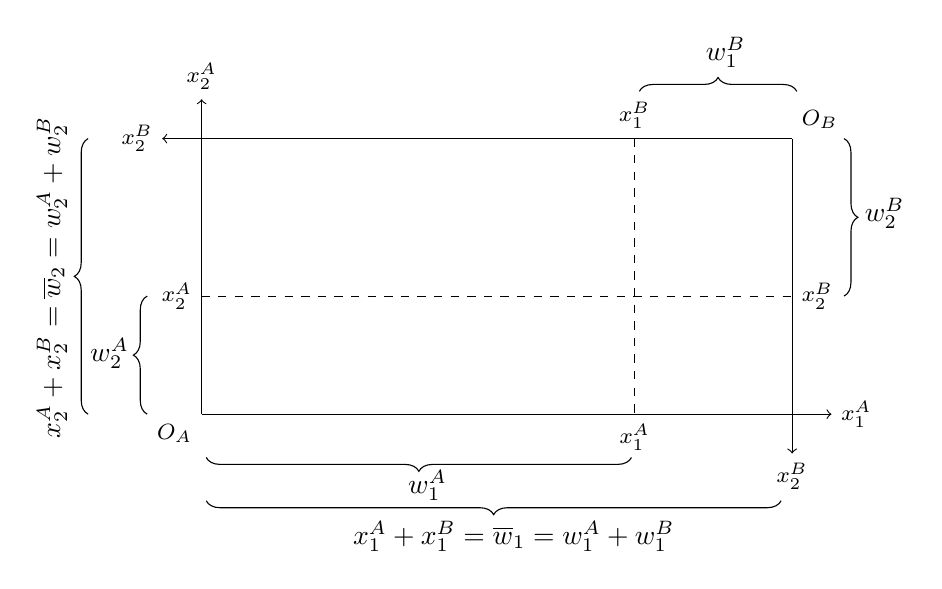
\begin{tikzpicture}[scale=1]
	% Formación de la caja
		% Consumidor A
			\draw[->] (0.5,0.5) node[align=center, below left] {\footnotesize $O_A$} -- (0.5,4.5) node[align=center, above] {\footnotesize $x_{2}^{A}$};
			\draw[->] (0.5,0.5) -- (8.5,0.5) node[align=center, right] {\footnotesize $x_{1}^{A}$};
	
		%Consumidor B
			\draw[->] (8,4) node[align=center, above right] {\footnotesize $O_B$} -- (0,4) node[align=center, left] {\footnotesize $x_{2}^{B}$};
			\draw[->] (8,4) -- (8,0) node[align=center, below] {\footnotesize $x_{2}^{B}$};
	
	% Intersección de una dotación
		\draw[dashed] (6,4) node[above] {\footnotesize $x_{1}^{B}$} -- (6,0.5) node[below] {\footnotesize $x_{1}^{A}$};
		\draw[dashed] (0.5,2) node[left] {\footnotesize $x_{2}^{A}$} -- (8,2)node[right] {\footnotesize $x_{2}^{B}$};
	
	% Llaves
		\draw [decorate,decoration={brace,amplitude=5pt},xshift=-4pt,yshift=0pt] (6.1,-0.05) -- (0.7,-0.05);
		\node [right] at (3,-0.4) {$w_{1}^{A}$};
	
		\draw [decorate,decoration={brace,amplitude=5pt},xshift=-4pt,yshift=0pt] (6.2,4.6) --(8.2,4.6);
		\node [right] at (6.78,5.1) {$w_{1}^{B}$};
		
		\draw [decorate,decoration={brace,amplitude=5pt},xshift=-4pt,yshift=0pt] (-0.05,0.5) --(-0.05,2);
		\node [left] at (-0.3,1.27) {$w_{2}^{A}$};
		
		\draw [decorate,decoration={brace,amplitude=5pt},xshift=-4pt,yshift=0pt] (8.8,4) --(8.8,2);
		\node [right] at (8.8,3.05) {$w_{2}^{B}$};
		
		\draw [decorate,decoration={brace,amplitude=5pt},xshift=-4pt,yshift=0pt] (8,-0.6) -- (0.7,-0.6);
		\node [right] at (2.3,-1.05) {$x_{1}^{A}+x_{1}^{B}=\overline{w}_1=w_{1}^{A}+w_{1}^{B}$};
		
		\draw [decorate,decoration={brace,amplitude=5pt},xshift=-4pt,yshift=0pt] (-0.8,0.5) --(-0.8,4);
		\node [left,rotate=90] at (-1.4,4.4) {$x_{2}^{A}+x_{2}^{B}=\overline{w}_2=w_{2}^{A}+w_{2}^{B}$};
\end{tikzpicture}
	\end{center}
\end{frame}
%------------------------------------------------
\begin{frame}{Segundo Teorema del Bienestar}
A través de un nuevo sistema de precios y una nueva dotación inicial
	\begin{center}
		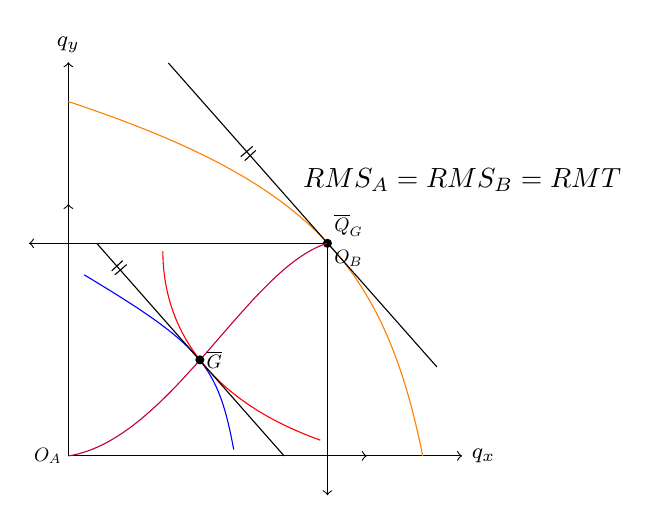
\begin{tikzpicture}
	% FPP
		% Ejes
			\draw[->] (10,0)-- (10,5) node[align=center, above] {\footnotesize $q_{y}$};
			\draw[->] (10,0) -- (15,0) node[align=center, right] {\footnotesize $q_{x}$};
		% Curva
			\draw [orange] (10,4.5) ..controls (13,3.5) and (14,2.5) .. (14.5,0);
			
	% Minicaja
		% Intersección
			\draw [<->] (9.5,2.7) -- (13.29,2.7) node [below right, scale=0.7] {$O_B$} -- (13.29,-0.5);
			\draw [<->] (10,3.2) -- (10,0) node [left, scale=0.7] {$O_A$} -- (13.79,0);
		% Puntos
			\draw[black, fill=black] (13.29,2.7) circle[radius=0.05] node [above right, scale=0.7] {$\overline{Q}_G$};
		% Curva de contrato
			\draw [purple] (10,0) ..controls (11.29,0.2) and (12.29,2.4) .. (13.29,2.7);
			\draw [blue] (10.2,2.3) ..  controls (11.7,1.4) and (11.9,1.15) .. (12.1,0.08);
			\draw [red] (11.2,2.6) ..  controls (11.2,1.6) and (11.8,0.7) .. (13.2,0.2);
		% Pendientes
			\draw (11.27,4.99) -- (14.68,1.13);
			\draw (10.36,2.7) -- (12.74,0);
		% Símbolo de paraleleas
			\draw (10.55,2.35) -- (10.69,2.48);
			\draw (10.59,2.3) -- (10.74,2.43);
			
			\draw (12.19,3.8) -- (12.34,3.93);
			\draw (12.24,3.75) -- (12.38,3.88);
		% 	Etqiueta
			\draw (15, 3.5) node {$RMS_A = RMS_B = RMT$};
		% Punto
			\draw[black, fill=black] (11.67,1.22) circle[radius=0.05] node [right, scale=0.7] {$\overline{G}$};
\end{tikzpicture}
	\end{center}
\end{frame}
%------------------------------------------------
\begin{frame}{Implicancia del Segundo Teorema del Bienestar}
	\begin{itemize}
		\item Se pueden \textbf{\textit{separar los problemas de}} distribución de los problemas de eficiencia.
		
		\item El mercado permite conseguir cualquier asignación de recursos que se desee: es \textbf{\textit{neutral desde el punto de vista distributivo}}.
		
		\item \textbf{\textit{Contenido normativo importante: Todo OP}} se puede sostener por un sistema de precios dada una redistribución adecuada de las dotaciones iniciales (implicancias para la Política Económica).
	\end{itemize}
\end{frame}